\chapter{\label{chapter:3_preliminaries}Preliminaries and Methodology}

This chapter will cover all the necessary tools required for the thesis. As we are considering asynchronous shared memory systems, the first section will describe the mathematical foundation for the computational model. This will describe formal concepts such as \emph{process}, \emph{algorithm}, and \emph{Linearizability}~\cite{DBLP_journals_toplas_HerlihyW90} in concurrent systems.

In the following section, we will explore the hardware foundations of concurrent systems. Specifically, we will discuss concepts such as \emph{cache memory}, \emph{consistency memory model}, \emph{cache coherence}, and \emph{memory fences}, which are crucial for correctly implementing concurrent algorithms. We will also discuss the concept of a memory model at the programming language level and examine the Java and C++ memory models that define the allowable behavior of multithreaded programs.

Finally, we will conclude this chapter by discussing the statistical experimental methodology used to analyze program implementations and compare performance between them.

\section{\label{sec:chapter-3:computation-model}Computation Model}

In the realm of computing, concurrent computation stands as a cornerstone for achieving efficient and scalable systems. It enables the execution of multiple tasks simultaneously, which is crucial for modern software applications such as web servers and programs exploiting multi-core processors' power. However, the complexity of concurrent systems requires precise mathematical models to reason about their behavior accurately. This section will discuss the mathematical model in detail, including its multiple components and assumptions for the essential topics developed in this thesis.

We consider the standard concurrent shared memory with \(n \ge 2\) \textit{asynchronous} processes, \(p_0, \ldots, p_{n-}\), which may \textit{crash} at any time during execution~\cite{DBLP_conf_spaa_Herlihy91,DBLP_books_daglib_0020056,DBLP_journals_toplas_HerlihyW90}. The \textit{index} of process \(p_i\) is \(i\). Processes communicate with each other by invoking \textit{atomic} instructions of base objects: either simple \R/\W, or more powerful \RMW, such as \SWAP or \CAS.

An \emph{algorithm} for a high-level concurrent object \(T\) (e.g., a queue or a stack) is a distributed algorithm \(\mathcal{A}\) consisting of local state machines \(A_1,\ldots, A_n\). Local machine \(A_i\) specifies which instruction of base objects execute to return a response when it invokes a (high-level) operation of \(T\); each of these instructions is a \emph{step}.

An \emph{execution} of \(\mathcal{A}\) is a (possibly infinite) sequence of steps, namely, instructions of base objects, plus invocations and responses of (high-level) operations of the concurrent object \(T\) with the following properties:

\begin{enumerate}
    \item Each process first invokes an operation, and only when it has a corresponding response can it invoke another operation, i.e., executions are well-formed and
    \item For any invocation to an operation \(op\) of a process \(p_i\), denoted as \(inv_i(op)\), the steps of \(p_i\) between that invocation and its correspondent response (if there is one), denoted \(res_i(op)\), are the steps specified by \(A_i\) when \(p_i\) invokes \(op\).
\end{enumerate}

An operation in an execution is \emph{complete} if both its invocation and response appear in the execution. An operation is \emph{pending} if only its invocation appears in the execution. It is assumed that after a process completes an operation, it non-deterministically picks the operation it executes next. An execution \(E\) is an \emph{extension} of an execution \(F\), if \(E\) is a prefix of \(F\), namely, \(E = F\cdot F'\) for some \(F'\).

For any finite execution \(E\) and any process \(p_i\), \(E|p_i\) denotes the sequence of invocations and responses of \(p_i\) in \(E\). Two finite executions \(E\) and \(F\) are equivalent if \(E|p_i = F|p_i\) \(\forall p_i\). For any execution \(E\), \(comp(E)\) denotes the execution obtained by removing from \(E\) all steps and invocations of pending operations.

A process is \emph{correct} in an infinite execution if it takes infinitely many steps. An implementation is lock-free if, in every infinite execution, infinitely many operations are complete~\cite{DBLP_journals_toplas_HerlihyW90}. An implementation is \emph{wait-free} if, in every infinite execution, every correct process completes infinitely many operations~\cite {DBLP_journals_toplas_Herlihy91}. Thus, a wait-free implementation is lock-free but not necessarily vice-versa. \emph{Bounded wait-freedom}~\cite{DBLP_conf_spaa_Herlihy91} additionally requires a bound on the number of steps needed to terminate. The \emph{step complexity} is the maximum number of steps a process needs to execute to return. The step complexity of an algorithm is the maximum among the step complexity of its operations.

In the \RAW{} synchronization pattern, a process first writes in a shared variable and then reads another shared variable, maybe executing other instructions in between. For example, this mechanism is widely used in the classic Lamport's bakery mutual exclusion algorithm (see~\cite {DBLP_books_daglib_0020056}). The correctness of the mechanism requires that the write and read instructions of a process are executed in a specific order, although there is no data dependence relation between them. In Section~\ref{sec:hardware-foundations}, we will discuss thoroughly how current processor architectures can reorder instructions, how they can alter the correctness of concurrent algorithms, and how to avoid this problem using \emph{fences}.

An algorithm, or one of its operations, is \emph{fence-free} if it does not require any specific ordering among its steps beyond what is implied by data dependence (e.g., the value written by a \W{} instruction depends on the value read by a previous \R instruction). Note that a fence-free algorithm does not use \RAW{} synchronization patterns. In our algorithms, we use notation \(\{O_1.inst_1, \ldots, O_x.inst_x\}\) to denote that the instructions \(O_1.inst_1, \ldots, O_x.inst_x\) can be executed in any order. Observe that memory fences (also known as memory barriers) are not required to correctly implement a fence-free algorithm in a concrete language or multi-core architecture since any reordering of non-data-dependent instructions does not affect the correctness of the algorithm.

\emph{Linearizability}~\cite{DBLP_journals_toplas_HerlihyW90} is the standard correctness condition for concurrent objects. Intuitively, an execution is linearizable if its (high-level) operations can be ordered sequentially, without reordering non-overlapping operations, so that their responses satisfy the specification of the implemented object.

A \emph{sequential specification} of a concurrent object \(T\) is a statute machine specified through a transition function \(\delta\). Given a state \(q\) and an invocation \(inv_i(op)\) of process \(p_i\), \(\delta(q, inv_i(op))\) returns the tuple \((q', res_i(op))\) (or a set of tuples if the machine is \emph{non-deterministic}) indicating that the machine moves to state \(q'\) and the response to \(op\) is \(res_i(op)\). The sequences of invocation-responses tuples \(\langle inv_i(op): res_i(op)\rangle\) produced by the state machine are its \emph{sequential executions}. For the sake of clarity, a tuple \(\langle inv_i(op): res_i(op)\rangle\) is simply denoted \(op\). Also, the subscripts of invocations and responses are omitted.

Given an execution \(E\), we write \(op <_E op'\) if and only if \(res(op)\) precedes \(inv(op')\) in \(E\). Two operations are \emph{concurrent} denoted \(op||_E op' \), if neither \(op <_e op'\) nor \(op' <_E op\). The execution is sequential if \(<_E\) is a total order.

\begin{definition}[Linearizability~\cite{DBLP_journals_toplas_HerlihyW90}]
Let be \(\mathcal{A}\) an algorithm for a concurrent object \(T\). A finite execution \(E\) of \(\mathcal{A}\) is \emph{linearizable with respect to \(T\)}, or just \emph{linearizable} if \(T\) is clear from the context, if there is a sequential execution \(S\) of \(T\) and \(E\) can be extended to an execution \(E'\) by appending zero or more responses such that:

\begin{enumerate}
    \item \(comp(E')\) and \(S\) are equivalent and
    \item for every two complete operations \(op\) and \(op'\) in \(E\), if \(op <_E op'\) then \(op <_S op'\).
\end{enumerate}

We say that \(\mathcal{A}\) \emph{is linearizable with respect to} \(T\) or just \emph{linearizable} if \(T\) is clear from the context if each of its executions is linearizable.
\end{definition}

Another correctness condition for concurrent objects is \emph{Set-Linearizability}. Set-Linearizability~\cite{DBLP_journals_jacm_CastanedaRR18, DBLP_conf_podc_Neiger94} is an extension of linearizability, allowing multiple operations to be linearized at the same linearization point, whereas linearizability requires a total order of operations.


A \emph{set-sequential specification} of a concurrent object differs from a sequential execution in that \(\delta\) receives as input the current state \(q\) of the machine and set \(Inv = \{inv_{id_1}(op_1), \ldots, inv_{id_t}(op_t)\}\) of operation invocations, and \(\delta(q, Inv)\) returns \((q', Res)\), where \(q'\) is the next state and \(Res = \{res_{id_1}(op_1), \ldots, res_{id_t}(op_t)\}\) are the responses to the invocations in \(Inv\) and each \(id_i\) denotes the index of the invoking/responding process. Intuitively , all operations \(op_1, \ldots, op_t\) are performed concurrently and move the machine from state \(q\) to \(q'\). The sequence of sets \(Inv\), \(Res\) is a \emph{concurrency class} of the machine. The state machine's sequences of concurrency classes are its \emph{set-sequential executions}. In our set-sequential specifications, invocations will be subscripted with the index of the invoking process only when there is more than one invocation in a concurrency class. Observe that a set-sequential specification in which all concurrency classes have a single element corresponds to a sequential specification.

Given a set-sequential execution S of a set-sequential object, the partial order \(<_S\) on the operations of \(S\) is defined as above: \(op <_S op'\) if and only if \(res(op)\) precedes \(inv(op')\) in \(S\), namely, the concurrency class of \(op\) appears before of the concurrency class of \(op'\).


\begin{definition}[Set-linearizability~\cite{DBLP_journals_jacm_CastanedaRR18, DBLP_conf_podc_Neiger94}]
    Let be \(\mathcal{A}\) an implementation of a concurrent object \(T\). A finite execution \(E\) of \(\mathcal{A}\) is \emph{set-linearizable with respect to} \(T\), or just \emph{set-linearizable} if \(T\) is clear from the context, if there is a set-sequential execution \(S\) of \(T\) and \(E\) can be extended to an execution \(E'\) by appending zero or more responses such that:

    \begin{enumerate}
        \item \(comp(E')\) and \(S\) are equivalent,
        \item for every two completed operations \(op\) and \(op'\) in \(E\), if \(op <_E op'\) then \(op <_S op'\).
    \end{enumerate}

    We say that \(\mathcal{A}\) is \emph{set-linearizable with respect to} \(T\), or just \emph{set-linearizable} if \(T\) is clear from the context if each of its executions is set-linearizable.
\end{definition}

\section{\label{sec:hardware-foundations}Hardware Foundations}

It is important to have knowledge of the hardware foundations behind concurrent computing besides the mathematical computation model. When we translate concurrent algorithms from the mathematical computation model to a program in a particular programming language, we need to deal with a lot of assumptions and rules that do not necessarily current processor architectures follow. For example, when we design our algorithms, we suppose linearizability as the correctness condition in asynchronous shared memory. Still, current processors cannot implement linearizability in the real world because this property incurs significant costs\footnote{For example, high power consumption, high manufacturing cost, low performance, etc.}. Instead of stronger correctness conditions for asynchronous shared memory, manufacturers provided distinct types of memory consistency (also known as memory model)~\cite{DBLP_series_synthesis_2020Nagarajan, DBLP_series_synthesis_2013Scott} for their processors and machines. A memory model is a precise, architecturally visible definition of shared memory correctness. Knowing about the hardware foundations helps us to implement correct algorithms. This will help us understand why specific tools like ``\emph{fences}'' are necessary to ensure correct concurrent computing. In this section, we will discuss the functioning of concurrent programs on computer hardware at a high level and focus on memory interactions at various levels.

\begin{figure}[ht!]
    \centering
    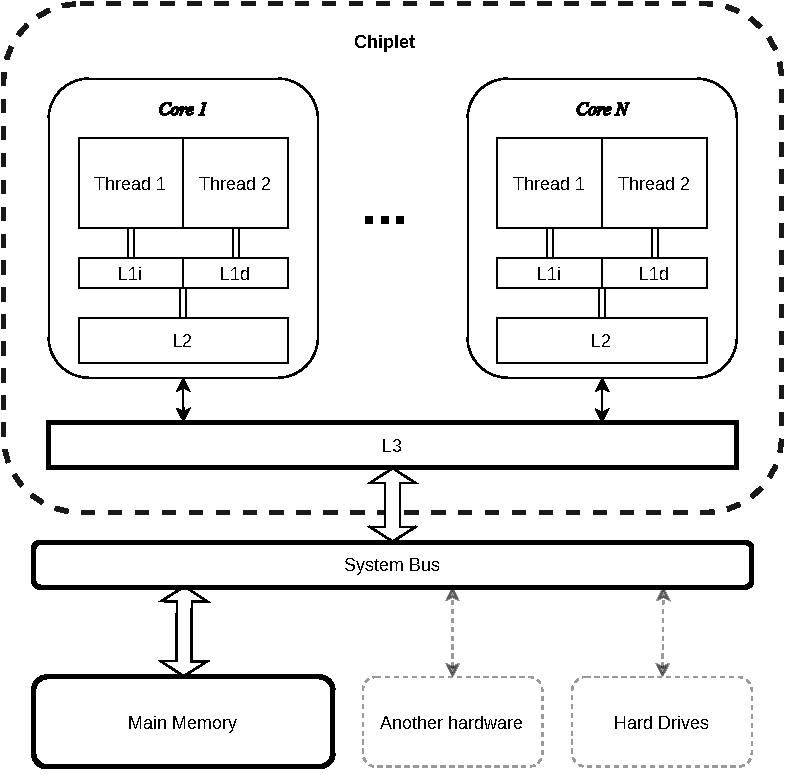
\includegraphics[width=0.7\linewidth]{contents//figures/III_2_cpu.pdf}
    \caption{Baseline model of a Multi-core Processor Chip.}
    \label{fig:multi-core-processor}
\end{figure}

When analyzing computer systems, it is important to consider those with multi-core processors communicate through a shared memory. This means all cores can perform loads and stores to all (physical) addresses in memory. A typical system model includes a single chip with multiple cores and off-chip main memory. You can see an illustration of this model in the figure~\ref{fig:multi-core-processor}\footnote{In the figure~\ref{fig:multi-core-processor}, we omit many features to simplify the reasoning about the hardware}. Usually, a multi-core processor includes \emph{cache memory}, a special high-speed memory close to the processor that allows fast process access. Caches decrease the average latency when accessing storage structures~\cite{DBLP_series_synthesis_2020Nagarajan, DBLP_series_synthesis_2013Scott}. In recent times, multi-core chips have adopted a three-tiered cache memory system. The first two levels, L1 and L2, are private to each core, while the third level, L3, is shared by all the cores. The primary purpose of L1 and L2 is to provide fast access to data and instructions for the core. Each core uses the first cache level to retrieve required data and execute instructions. Cache L1 is divided into two sub-caches, one for data (L1d) and the other for instructions (L1d). Typically, access to this cache level is faster than access to other levels. The second level of cache is usually more extensive and stores data and instructions about to be executed.
Multiple cores share the third cache level and serve as a source for the L2 cache~\cite{devices_amd64,guideintel}.


The \emph{main memory} holds frequently accessed data for the CPU, such as instructions or processing data, and allows faster access than secondary memory. The processor calls the \emph{memory bus} to obtain such data and instructions, which transfers data from the primary memory to the CPU and cache memory. This bus has two parts: the data bus and the address bus. The data bus transfers information between the primary memory and the corresponding chipset. On the other hand, the address bus is used to retrieve information about the location of stored data.


When considering the simplified view of cache and memory architecture, it is important to ensure that shared memory is correct. Incoherence can occur when multiple actors have concurrent access to caches and memory, such as processor cores, external devices, system buses, etc., which may read and/or write to them. To us, the cores will be the main actors, but we must consider the possibility of other actors interacting with caches and memory.

In order to ensure that shared memory is accurate, two important issues must be addressed: \emph{consistency} and \emph{correctness}. Consistency provides guidelines for memory reads and writes and how they act upon memory. These rules must take into account the behavior of these operations when multiple threads or even a single thread accesses memory. Consistency models define the proper behaviors for shared memory with regard to loads and stores and do not reference caches or coherence~\cite{DBLP_series_synthesis_2020Nagarajan}. Memory consistency models (or memory models) specify shared memory correctness. They define the allowed behaviors for multithreaded programs that execute with shared memory. The most intuitive and strongest memory model is \emph{Sequential Consistency} (SC)~\cite{lamport1979how}. Another memory model used by systems \emph{x86} and \emph{SPARC} is \emph{Total Store Order} (TSO) ~\cite{DBLP_conf_tphol_OwensSS09, DBLP_journals_cacm_SewellSONM10, sparc1992sparc}. TSO is motivated by the desire to use \emph{first-in-first-out} write buffers to hold the results of committed stores before writing results to the caches. Additionally, ``relaxed'' or ``weak'' memory models are considered because they show that most memory orderings in strong models are unnecessary~\cite{DBLP_series_synthesis_2020Nagarajan}.


It is important to consider cache coherence protocols when dealing with caching and solving coherence issues. These protocols come into play when multiple cores access multiple copies of data, with at least one being a write access. To ensure that the data accessed is up-to-date and consistent, the distributed set of cores implements a set of rules within a system~\cite{DBLP_series_synthesis_2020Nagarajan}. Hence, it is essential to consider consistency models and cache coherence protocols to prevent access to stale or incoherent data. The goal of a coherence protocol is to maintain coherence by enforcing the next invariants~\cite{DBLP_series_synthesis_2020Nagarajan}:

\begin{enumerate}
  \item \emph{Single Writer, Multiple-Read Invariant} \texttt{(SWMR)}. At any given
 (logical) time, only one core may write to memory location \(A\). Other cores may only read the memory location \(A\).

  \item \emph{Data-Value Invariant}. The value of the memory location at the beginning of an epoch is the same as the value of the memory location at the end of its last read-write epoch.
\end{enumerate}

To ensure that the \texttt{SWMR} and \emph{data value} invariants are always maintained, we use a distributed system consisting of a collection of \emph{coherence controllers}. Such controllers are finite state machines associated with each storage structure (cache and memory). These coherence controllers exchange messages with each other to ensure that invariants are upheld for each structure. The coherence protocol specifies the interaction between these finite-state machines and moving from one state to another based on the conditions of the data and the cache memory.
Coherence states play a crucial role in ensuring that the system operates smoothly. The most commonly used coherence states are modified (M), shared (S), and invalid (I). However, AMD has gone a step further with its MOESI protocol~\cite{devices_amd64} and introduced two additional states, owned (O) and exclusive (E), to improve the system's efficiency. On the other hand, Intel has created its extension called MESIF~\cite{guideintel} to achieve the same goal.

\section{About Fences And Its Use In Concurrent Algorithms}

Processors that support the TSO memory model do not guarantee ordering between a store and a subsequent load that comes after it in program order. However, they ensure that the load gets the value of the earlier store.  To order these instructions, the programmer must explicitly specify that ordering by inserting a \emph{fence} instruction between the store and the subsequent load.
%The \emph{fence} instruction ensures that all instructions before it in program order are executed before any instructions after it in program order.
A \emph{memory fence} is a barrier instruction that causes a CPU or compiler to enforce an ordering constraint on memory operations (loads and stores) issued before and after the barrier instruction. These instructions are necessary because most modern CPUs or compilers employ performance optimizations, changing the order of the instructions on one program, which could result in out-of-order execution. Typically, these optimizations are unnoticed in a single-thread program but can cause unpredictable behavior in concurrent programs (See Example~\ref{ex:reordering}).

\begin{example}[Instruction re-ordering]
\label{ex:reordering}
Consider the following multi-thread program with two threads, each concurrently running on distinct cores. The first thread executes the code shown in~\ref{lst:thread1}, and the second one executes the code shown in~\ref{lst:thread2}:

\begin{lstlisting}[language=c++,label={lst:thread1}, caption={Code execute by thread 1 on core 1} ,captionpos=b]
while (z == 0);
print(y);
\end{lstlisting}

\begin{lstlisting}[language=c++,label={lst:thread2} ,caption={Code executed by thread 2 on core 2} ,captionpos=b]
y = 30;
z = 1;
\end{lstlisting}


In this case, we might expect that the instruction \texttt{print(y)} always prints the number 30. Nevertheless, the compiler or the CPU could change the order of the instructions for thread 2, giving, as a result, an execution where the value for \texttt{y} is \emph{undefined}, and the instructions could be interleaved as shown in the code~\ref{lst:reordering}:

\begin{lstlisting}[language=c++,label={lst:reordering},caption={Code reordered by CPU}, captionpos=b]
z = 1; // Thread 2
while (z == 0); // Thread 1
print(y); // Thread 1
y = 30; // Thread 2
\end{lstlisting}

However, this execution is sequentially consistent but is an out-of-order execution producing an undefined result. With the use of memory barriers, we can ensure that instructions do not be reordered. For example, our code could be rewritten as shown in~\ref{lst:thread1-fence} and~\ref{lst:thread2-fence}:

\begin{lstlisting}[language=c++,label={lst:thread1-fence} ,caption={Updating code~\ref{lst:thread1} to use fences.} ,captionpos=b,numbers=none]
while (z == 0);
fence();
print(y);
\end{lstlisting}

\begin{lstlisting}[language=c++,label={lst:thread2-fence},caption={Updating code~\ref{lst:thread2} to use fences.} ,captionpos=b,numbers=none]
y = 30;
fence();
z = 1;
\end{lstlisting}

\end{example}

\section{After Hardware Foundations, What's Up About Programming Languages?}

The previous section introduces the hardware foundations necessary to understand the memory consistency models and the cache protocols to implement correct concurrent programs. The model presented in the previous section is placed at the hardware level and low-level software. However, it is also important to (re)define memory models for high-level languages because it defines an interface between a program and any hardware or software that may transform that program. Also, a memory model helps to reason about how the program will behave in a multi-core environment~\cite{DBLP_journals_cacm_AdveB10, DBLP_series_synthesis_2020Nagarajan}.

In recent years, memory models have been specified for C++~\cite{DBLP_conf_pldi_BoehmA08} and Java~\cite{DBLP_conf_popl_MansonPA05}, which are two of the most used programming languages currently. These programming language memory models describe the expected behavior of language-level threads, locks, atomics, and Read-Modify-Write instructions. Also, these memory models help to specify what high-level language authors should expect and what implementors of compilers, runtime systems, and hardware may do. Figure~\ref{fig:memory-models} illustrates the difference between (a) high-level and (b) low-level memory models.

\begin{figure}[ht!]
    \centering
    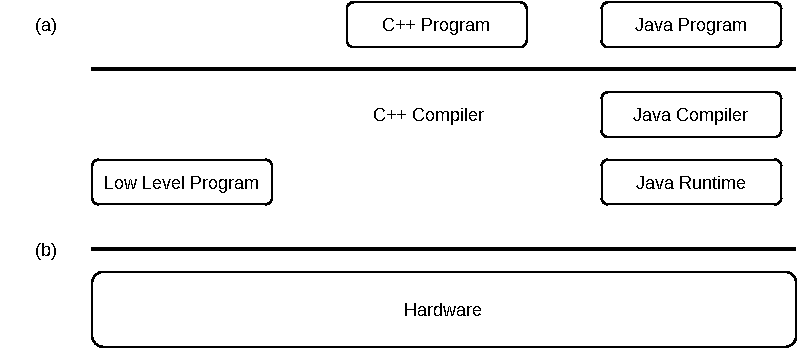
\includegraphics[width=0.9\linewidth]{contents//figures/III_3_memory_model.pdf}
    \caption{(a) High-level language and (b) hardware memory models.}
    \label{fig:memory-models}
\end{figure}

Java and C++ adopt the relaxed memory model approach of ``\emph{Sequential Consistency for Data-Race Freedom (SC for DRF)}''~\cite{DBLP_conf_isca_AdveH90}.  A data race occurs when two memory accesses target the same location simultaneously and are not reads or synchronization operations. The approach of \emph{SC for DRF} guarantees that a program is correctly synchronized if and only if all sequentially consistent executions are free of data races. If a program is correctly synchronized, then all program executions will appear to be sequentially consistent~\cite{javamemorymodelspec}. It is important to note that according to the C++ specification, there is a possibility of having valid programs that use synchronization operations with a memory order other than \texttt{memory\_order\_seq\_cst}. In such cases, the resulting program may be correct, but there is no guarantee of sequential consistency~\cite{DBLP_conf_pldi_BoehmA08}. In both cases, reordering or eliminating memory accesses between synchronization accesses is allowed for performance as long as data-race-free programs obey Sequential Consistency~\cite{DBLP_series_synthesis_2020Nagarajan}.

The memory order in C++ determines how memory is accessed~\cite{memoryOrderCpp2020}. It ensures that regular, non-atomic memory accesses are ordered around atomic operations. In a multi-core system, where multiple threads read and write to several variables simultaneously, one thread may observe the values changing in a different order than the order in which another thread wrote them. This can cause the apparent order of changes to differ among multiple reader threads~\cite{memoryOrderCpp2020}. Similar effects can occur even on uniprocessor systems due to compiler transformations allowed by the memory model. By default, all atomic operations in the library follow a sequentially consistent ordering. However, this default approach can negatively impact performance. To mitigate this, the atomic operations in the library can be provided with an additional \texttt{std::memory\_order} argument. This argument specifies the precise constraints the compiler and processor must enforce for a given operation beyond just ensuring atomicity~\cite{memoryOrderCpp2020}. Six memory models are defined in the specification, ranging from the weakest model (\texttt{memory\_order\_relaxed}) to the strongest one (\texttt{memory\_order\_seq\_cst}).

At the end of the previous section, we discussed about memory fences. C++ and Java provide memory fences to implement correct concurrent programs. C++ provides the function \texttt{atomic\_thread\_fence}, which establishes memory synchronization ordering of non-atomic and relaxed atomic accesses as instructed by order, without an associated atomic operation. A note about \texttt{atomic\_thread\_fence} functions is that on x86 (x86\_64), these functions issue no CPU instructions and only affect compile time code, with the exception for \texttt{std::atomic\_thread\_fence(std::memory\_order::seq\_cst)}, which issue the full memory fence instruction \texttt{MFENCE}.

In the case of Java, the latest versions provide the class \texttt{VarHandle}\footnote{\texttt{java.lang.invoke.VarHandle}}, which exposes the memory fence methods~\cite{varHandleJdk92017} shown in the table~\ref{table:fences}. Many of these fences try to be similar to those defined by the specification of C++.

\begin{table}[ht!]
\begin{tabular}{@{}ll@{}}
\toprule
\multicolumn{1}{l}{\textbf{Fence}} & \textbf{Description} \\ \midrule
\texttt{fullFence} & \begin{tabular}[c]{@{}l@{}}Ensures that loads and stores before the fence will \\not be reordered with loads and stores after the fence.\\ This method has memory ordering effects compatible with \\  \texttt{atomic\_thread\_fence(memory\_order\_seq\_cst)}.\end{tabular} \\
\midrule
\texttt{acquireFence} & \begin{tabular}[c]{@{}l@{}}Ensures that loads before the fence will not be reordered\\ with loads and stores after the fence. This method has\\ memory ordering effects compatible with \\\texttt{atomic\_thread\_fence(memory\_order\_acquire)}.\end{tabular} \\
\midrule
\texttt{releaseFence} & \begin{tabular}[c]{@{}l@{}}Ensures that loads and stores before the fence will\\ not be reordered with stores after the fence. \\ This method has memory ordering effects compatible with\\  \texttt{atomic\_thread\_fence(memory\_order\_release)}.\end{tabular} \\
\midrule
\texttt{loadLoadFence} & \begin{tabular}[c]{@{}l@{}}Ensures that loads before the fence will\\ not be reordered with loads after the fence.\end{tabular} \\
\midrule
\texttt{storeStoreFence} & \begin{tabular}[c]{@{}l@{}}Ensures that stores before the fence will\\ not be reordered with stores after the fence.\end{tabular} \\ \bottomrule
\end{tabular}
\caption{\label{table:fences}Memory fences provided by Java}
\end{table}

%\subsection{Memory management}
%\label{sec:org1ca9ee9}

%To implement efficiently the idempotent algorithms in an environment without garbage collection, it's necessary to use some technique or methodology to provide garbage collection when atomic pointers are used or when distinct threads want to reclaim the memory of the object associated with the pointer.

%\begin{enumerate}
%\item Strategies to delete shared pointers
%\label{sec:org36ce5a6}

%\begin{itemize}
%\item Add pointers to list to safety delete.
%\item Do this when there aren't more threads accessing methods.
%\begin{itemize}
%\item Increase the counter when a thread enters the method and decrease when
%it exits.
%\item Delete all pointers when the counter is equal to zero.
%\end{itemize}
%\end{itemize}


%\item Hazard pointers
%\label{sec:org3992578}

%The \emph{Hazard Pointers} is a technique to manage language memory without garbage collectors. Maged proposed this technique Michael \cite{DBLP_journals_tpds_Michael04}. They are so-called because deleting a pointer that might be referenced by other thread(s) is dangerous. If another thread keeps holding references to that pointer and proceeds to access that pointer after being deleted, you have an undefined behavior \cite{DBLP_journals_tpds_Michael04}.

%The basic idea of this technique is the following:

%\begin{itemize}
%\item If a thread wants to use a pointer that another thread might want to delete, it first sets a hazard pointer to the pointer, informing the other thread that deleting it would be dangerous. Once the object is no longer needed, the hazard pointer is cleared.
%\item When a thread wants to delete the pointer, it must check if the hazard pointers belong to the other threads in the system. If no one has a reference to the pointer, then it's safe to delete it. Otherwise, it must be left until later.
%\item Periodically, we must check the list of objects left until later to see if any of them can be deleted now.
%\end{itemize}

%A general pseudocode for this technique could be the following:

%\begin{lstlisting}[language=c++,label= ,caption= ,captionpos=b,numbers=none]
%void func() {
%    std::atomic<void*>& hp = get_hazard_pointer_for_current_thread();
%    void* old_data = data.load();
%    do {
%        void* temp;
%        do{ // Loop until you've set the hazard pointer
%            temp = old_data;
%            hp.store(old_data);
%            old_data = data.load();
%        } while (old_data != temp);
%          }while (old_data &&
%            !data.compare_exchange_strong(old_data, old_data->next);
%    // Do something with old_data
%    hp.store(nullptr); // clearing usage of hazard pointer
%    // Trying clearing
%    if (outstanding_hazard_pointers_for(old_head))
%    {
%        reclaim_later(old_data);
%    }
%    else
%    {
%        delete old_data;
%    }
%    delete_nodes_with_no_hazards();
%}
%\end{lstlisting}


%\item Atomic Smart Pointers (Herlihy, Chapter 19) (Not available for GCC and CLang)
%\label{sec:org58c7cdb}


%When a memory region is reclaimed, the programmer cannot know how that region of memory will be reused or whether it will be reused. We need a way of developing a (general) solution to prevent the sorts of races when a memory region is reclaimed by many threads asynchronously. We can do this by delaying reclamation. Considering pending operations on a concurrent data structure, a sufficient condition is that \emph{memory is only reclaimed when it is impossible for any pending operation to access in the future}.

%This property could also be achieved by \emph{reference counting}. In a reference counted implementation of a data structure (like a list), a counter of type atomic<int> is associated with each node. Whenever a reference to node N is created
%\end{enumerate}

\section{\label{sec:methodology}Experimental Methodology}

One of the goals of this thesis is to assess our algorithms' performance. In experimental computer science research and development, benchmarking plays a vital role. Developers perform benchmarking tests on their products under development to evaluate their performance, while researchers use benchmarking to assess the impact on the performance of their novel research ideas~\cite{DBLP_conf_oopsla_GeorgesBE07}.

In this thesis, we have followed and adapted the guidelines presented in the following sources \cite{forsyth2018probability, DBLP_conf_oopsla_GeorgesBE07,lilja2005measuring}. These guidelines provide fundamental techniques for measuring computer performance and strategies for analyzing and interpreting the resulting data. Topics covered include performance metrics, benchmarking programs, and statistical tools. By following these guidelines, we can perform rigorous statistical evaluation, better understand the performance of our algorithm implementations, and compare them against other algorithms.

A common method of evaluating experimental results is by measuring performance or throughput. But what do these terms mean? \emph{Throughput}, as defined by the Cambridge Dictionary, is the amount of work completed in a given period. In contrast, \emph{performance} refers to how well something functions or works. Specifically, performance is measured by the amount of useful work a system accomplishes, typically determined by its accuracy, efficiency, and speed of executing instructions. One or more of the following factors might be involved when performance is measured:

\begin{enumerate}
\item Short response time for a given piece of work.
\item High throughput.
\item Low utilization of computing resources.
\item High availability of a computing system.
\item High bandwidth.
\item Short data transmission time.
\end{enumerate}

From the work of Lilja~\cite{lilja2005measuring}, some strategies for measurement are:

\begin{itemize}
\item \textbf{Event driven}: It records the information necessary to calculate the
performance metric whenever an event occurs.
\item \textbf{Tracing}: Similarly to the previous, but instead of recording the event
that has occurred, a portion of the system is recorded to identify the event.
\item \textbf{Sampling}: This strategy records a portion of the system in a fixed time
interval.
\item \textbf{Indirect measurement}: This type occurs when the metric data is not
directly accessible, and you must find another metric that can be measured
directly.
\end{itemize}

We can combine those strategies with interval timers to measure how long it takes to execute the program or some section of code, providing a time basis for sampling.


%\hl{To begin with a performance-analysis problem, three techniques can be used to find the desired solution:}

%\begin{enumerate}
%\item Measurements of existing systems.
%\item Simulation.
%\item Analytical modeling.
%\end{enumerate}

\subsection{\label{subsec:statistics}Statistic tools for experiments}

As computer science researchers, we aim to measure and compare the performance of novel and existing algorithms. To evaluate the effectiveness of these algorithms, we need to establish an experimental methodology that allows us to measure their performance and throughput and determine whether they are competitive. This thesis proposes various versions of the same algorithm for different studies. We will divide our experiments into two categories. The first category is related to measuring the performance of the different algorithm versions.
In contrast, the second category is focused on comparing our best algorithm (or the two best) to other algorithms in the literature. To evaluate the performance of our algorithms, we will measure the time required to execute a set of operations over a given interval of time, i.e., this will help us determine how quickly the program can complete its execution. The technique used to measure the time of an event is the following:

\begin{itemize}
\item Read the current time and store it in a variable \texttt{start\_count}.
\item Let the portion of the program execute.
\item Read the current time and store it in a variable \texttt{stop\_count}.
\item Take the difference between \texttt{start\_count} and \texttt{stop\_count}. This will be the
total time required to execute the event.
\end{itemize}

This technique for measuring the execution time of any portion of a program
is known as the \emph{wall clock} time~\cite{lilja2005measuring}. We will use this technique to measure all the events we want to track. However, remember that this measurement includes time spent on other system operations, such as memory paging, thread interleaving, input/output operations, and network communication, if applicable. These external events can introduce uncertainty, errors, or noise into our measurements. To quantify the uncertainty, we need to use probability and statistics tools. To summarize a collection of measures, we can use indices of central tendency such as the mean, median, and mode. The most commonly used index is the sample arithmetic mean or average, which can summarize all the measurements into a single value that represents the center of the distribution of these values.  To quantify the precision of our measurements, we can use a \emph{confidence interval} for the mean value~\cite{DBLP_conf_oopsla_GeorgesBE07, lilja2005measuring}. Other tools we need are the \emph{sample variance}, the \emph{standard deviation}, and the \emph{coefficient of variation}.

Formally, the \emph{(sample arithmetic) mean} is defined to be:

\begin{equation}
\bar{x}_A = \frac{1}{n}\sum^n_{i = 1}x_i
\end{equation}

Where \(x_i\) values are the individual measurements. The \emph{sample variance}
represent our calculated estimate of the actual variance. It is defined to be:

\begin{equation}
s^2 = \frac{\sum_{i = 1}^n(x_i - \bar{x}^2)}{n - 1}
\end{equation}

Where the \(x_i\) are the \(n\) independent measurements and \(\bar{x}\) is
the corresponding sample mean. From the previous equation, the standard
deviation is defined as the positive square root of the variance:

\begin{equation}
s = \sqrt{s^2} = \sqrt{\frac{\sum_{i = 1}^n(x_i - \bar{x}^2)}{n - 1}}
\end{equation}

The coefficient of variation (COV) is defined to be:

\begin{equation}
  COV = \frac{s}{\bar{x}}
\end{equation}

Suppose we can approximate the distribution of random errors by a Gaussian
distribution. In that case, we determine how well our estimate of the true value is concerning the actual true value using the properties of the distribution. We use
confidence intervals to find a range of values with a probability
of including the true value. To do that, we must consider two cases:

\begin{enumerate}
\item When the number of measurements is large \((n \ge 30)\).
\item When the number of measurements is small \((n < 30)\).
\end{enumerate}

For the first case, we use the sample mean \((\bar{x})\) as the best
approximation of the true value. If the \(n\) samples used to calculate
\(\bar{x}\) are all independents with mean \(\mu\) y standard deviation
\(s\), the central limit theorem then assures us that, for large values of
\(n\), the sample mean \(\bar{x}\) is approximately Gaussian distributed with
mean \(\mu\) and standard deviation \(s / \sqrt{n}\). We can quantify the
precision of the measurements searching two values \(c_1\) and \(c_2\), such
that the probability of the mean value being between those two values is \(1 -
   \alpha\). That is \(PR[c_1 \le \bar{x} \le c_2] = 1 - \alpha\). \(c_1\) and
\(c_2\) are chosen to form a symmetric interval around \(\bar{x}\) such that
\(Pr[x < c_1] = Pr[x > c_2] = \frac{\alpha}{2}\). The interval \([c_1, c_2]\)
is called \textit{confidence interval} for \(\bar{x}\) and \(\alpha\) is
called the \textit{significance level} and the value \((1 - \alpha)\) is
called the \textit{confidence level}. From the central limit theorem, we
have:

\begin{equation}
c_1 = \bar{x} - z_{1 - \alpha/2}\frac{s}{\sqrt{n}}
\end{equation}
\begin{equation}
c_2 = \bar{x} + z_{1 - \alpha/2}\frac{s}{\sqrt{n}}
\end{equation}

where \(\bar{x}\) is the sample mean, \(s\) is the sample standard deviation,
\(n\) is the number of measurements and \(z_{1 - \alpha/2}\) is the value of
a standard unit normal distribution with mean \(\mu = 0\) and variance
\(s^2\), which obeys the following property: \(Pr[Z \le z_{1-\alpha/2}] =
   1 - \alpha/2\), where the value \(z_{1 - \alpha/2}\) is typically obtained
from a pre-computed table.

In the second case, for a small number of measurements \((n < 30)\), the
sample variances \(s^2\) calculated for different groups of measurements can
vary significantly. The distribution of the transformed value \(z =
   \frac{\bar{x} - x}{s/\sqrt{n}}\) follows the \emph{Student's} \emph{t}-distribution
with n - 1 degrees of freedom. Then, the confidence interval for \(\bar{x}\)
when \(n < 30\) can be computed as:

\begin{equation}
c_1 = \bar{x} - t_{1-\alpha/2;n-1}\frac{s}{\sqrt{n}}
\end{equation}
\begin{equation}
c_2 = \bar{x} + t_{1-\alpha/2;n-1}\frac{s}{\sqrt{n}}
\end{equation}

where \(t_{1 - \alpha/2;n-1}\) defined such that a random variable \(T\) that
follows the \emph{Student's t}-distribution with \(n - 1\), obeys: \(Pr[T < t_{1 -
   \alpha/2;n - 1}] = 1 - \alpha/2\), where the value \(z_{1 - \alpha/2;n - 1}\)
is typically obtained from a pre-computed table.

Confidence intervals are an interesting concept because they provide insight into how much noise there is in measurements. However, when making decisions about the performance of one or more systems, we need to determine whether changes are due to random fluctuations or if they are statistically significant. To do this, we can use the following two techniques~\cite{DBLP_conf_oopsla_GeorgesBE07, lilja2005measuring}:

\begin{enumerate}
\item Comparing two alternatives
\item Analysis of variance (ANOVA)
\end{enumerate}

The first technique is simple. The approach to comparing two alternatives is
to determine whether the confidence intervals for two groups of measurements
overlap. If the intervals do not overlap, we can conclude that there is no
evidence to suggest that there is not a statistically significant
difference. In another case, we cannot conclude that the differences seen in
the mean values are not due to random fluctuations. To determine whether
there is no statistical difference, we need to calculate the confidence
interval for the difference of the means of the two alternatives. First
determine the sample mean \(\bar{x_1}\) and \(\bar{x_2}\) and the sample
standard deviation \(s_1\) and \(s_2\). Then, compute the difference of the
means as \(\bar{x} = \bar{x_1} - \bar{x_2}\). The standard deviation \(s_x\)
of the difference of the mean values is computed as:

\begin{equation}
  s_x = \sqrt{\frac{s_1^2}{n_1} + \frac{s_2^2}{n_2}}
\end{equation}

Then, the confidence interval for the difference of the means is then given
by:

\begin{equation}
  c_1 = \bar{x} - z_{1 - \alpha/2}s_x
\end{equation}

\begin{equation}
 c_2 = \bar{x} + z_{1 - \alpha/2}s_x
\end{equation}

The confidence interval calculated before is in the case when the number of
measurements is considerable on both systems, i.e., \(n_1 \ge 30\) and \(n_2
   \ge 30\). When the number of measurements on at least one of the systems is
smaller than 30, we can no longer assume that the difference between the means is
under Gaussian distribution. In the last case, when the number of
measurements in both systems is small, i.e., \(n_1 < 30\) and \(n_2 < 30\),
we need to resort to the Student's \emph{t} distribution by replacing the value
\(z_{1 - \alpha/2}\) with \(t_{1 - \alpha/2;n_{df}}\), where \(n_{df}\)
represent the degrees of freedom, which it can approximate by integer number
nearest to:

\begin{equation}
 n_{df} = \frac{(\frac{s_1^2}{n_1} + \frac{s_2^2}{n_2})^2}{\frac{(s_1^2/n_1)^2}{n_1 - 1} + \frac{(s_2^2/n_2)^2}{n_2 - 1}}
\end{equation}

In the case of the \textbf{Analysis of Variance (ANOVA)}, a general technique
for observing the variation in a collection of measurements into meaningful
components. To perform this analysis, it is necessary to assume that the errors
in the measurements for the distinct alternatives are independent and under
normal distribution. The variance for the measurement errors is the same
for all alternatives. The variation observed is divided into:

\begin{enumerate}
\item The variation observed \emph{within} each system is assumed caused by the
measurement error.
\item The variation \emph{between} alternatives.
\end{enumerate}

If the variation between the alternatives is larger than the variation within each alternative, then it can be concluded that there is a statistically significant difference between the alternatives. To evaluate ANOVA, we must organize the measurements as shown in the table~\ref{table:anova}: there are \(n \cdot k\) measurements for all \(k\) alternatives. The column means are defined as:

\begin{equation}
  \bar{y}_{.j} = \frac{\sum^n_{i = 1}y_{ij}}{n}
\end{equation}


\begin{table}
\begin{center}
\begin{tabular}{|l|l|l|l|l|l|l|l|}
\hline
Measurements & 1 & 2 & \(\hdots\) & \(j\) & \(\hdots\) & \(k\) & Overall mean\\[0pt]
\hline
1 & \(y_{11}\) & \(y_{12}\) & \(\hdots\) & \(y_{1j}\) & \(\hdots\) & \(y_{1k}\) & \\[0pt]
2 & \(y_{21}\) & \(y_{22}\) & \(\hdots\) & \(y_{2j}\) & \(\hdots\) & \(y_{2k}\) & \\[0pt]
\(\vdots\) & \(\vdots\) & \(\ddots\) & \(\hdots\) &  &  &  & \\[0pt]
\(i\) & \(y_{i1}\) & \(y_{i2}\) & \(\ddots\) & \(y_{ij}\) & \(\vdots\) & \(y_{ik}\) & \\[0pt]
\(\vdots\) & \(\vdots\) & \(\vdots\) & \(\vdots\) & \(\ddots\) &  &  & \\[0pt]
\(n\) & \(y_{n1}\) & \(y_{n2}\) & \(\hdots\) & \(y_{nj}\) & \(\hdots\) & \(y_{nl}\) & \\[0pt]
\hline
Column means & \(\bar{y}_{.1}\) & \(\bar{y}_{.2}\) & \(\hdots\) & \(\bar{y}_{.j}\) & \(\hdots\) & \(\bar{y}_{.k}\) & \(\bar{y}_{..}\)\\[0pt]
\hline
\end{tabular}
\end{center}
\caption{\label{table:anova}Organizing the \(n\) measurements for \(k\) alternatives in an ANOVA analysis}
\end{table}

The overall mean is defined as:

\begin{equation}
  \bar{y}_{..} = \frac{\sum^k_{j = 1}\sum^n_{i = 1}y_{ij}}{n\cdot{}k}
\end{equation}

Compute the sum of squares of the differences between the mean of the measurements for each alternative and the overall mean to find the variation due to the effects of the alternatives (SSA):

\begin{equation}
    SSA = n \sum_{j = 1}^{k} (\bar{y}_{.j} - \bar{y}_{..})^2
\end{equation}

The variation within an alternative due to random effects is calculated by summing the differences (or errors) between individual measurements and their respective alternative mean.

\begin{equation}
    SSE = \sum_{j = 1}^{k}\sum_{i = 1}^{n} (y_{ij} - \bar{y}_{.j})^2
\end{equation}

Finally, the sum-of-squares total, SST, or the sum of squares of the differences between the individual measurements and the overall mean is defined as:

\begin{equation}
    SST = \sum_{j = 1}^{k}\sum_{i = 1}^{n} (y_{ij} - \bar{y}_{..})^2
\end{equation}

It is possible to split the observed total variation (SST) into a \emph{within} component (SSE) and a \emph{between} component (SSA).

\begin{equation}
    SST = SSA + SSE
\end{equation}

ANOVA analysis quantifies whether there is a difference in variation across alternatives (SSA) compared to variation within each alternative (SSE) due to random measurement errors. One way to do this is to compare the fractions \(\frac{SSA}{SST}\) and \(\frac{SSE}{SST}\). A more rigorous approach is to use the F-test~\cite{lilja2005measuring}, which tests whether two variances are significantly different.  After conducting an ANOVA test, we may determine a significant difference between the alternatives, but the test does not specify which alternatives have a significant difference. Various techniques can be employed to determine whether there is a statistically significant difference between alternatives. We will describe the techniques we'll use for each of our specific case studies.

\subsection{\label{subsec:stat-rigor-meth}Statistically rigorous methodology}

Measuring performance in programming languages like Java is far from trivial due to the many factors that can affect the computation, e.g., the garbage collector and heap size. We use the methodology proposed by Georges, Buytaert, and Eeckhout~\cite{DBLP_conf_oopsla_GeorgesBE07} to obtain statistically rigorous results. The methodology measures the \textit{steady-state} performance, which concerns long-running applications in which start-up is of less interest. The methodology is as follows for a given experiment:


\begin{enumerate}
\item First, the experiment is executed at most 30 times.
  \begin{itemize}
  \item Among the executions, it is determined the first one \(s_i\) where the steady-state performance is reached. This means that the \textit{coefficient of variation} (CoV)~\footnote{CoV is the standard deviation \(s\) divided by the mean \(\bar{x}\).} of the most recent five {executions} falls below an established threshold (0.02). If the CoV never drops below the threshold established for any five consecutive {executions}, it is considered the five consecutive {executions} with the lowest CoV.
  \item The mean \(\bar{x}_i\) of the last five {executions} under steady-state is:
    \begin{equation*}
      \bar{x}_i = \frac{\sum^{s_i}_{j=s_i - k}x_{ij}}{5}
    \end{equation*}
  \end{itemize}
\item Second, it is computed the confidence interval by performing 15 {executions} with \(95\%\) confidence interval over the \(\bar{x_i}\) measurements.

\end{enumerate}

Since the number of measurements is small, the confidence interval is computed under the assumption that the distribution of the transformed value \(t\) corresponds with:
\begin{equation*}
  t = \frac{\bar{x} - \mu}{s/\sqrt{n}}
\end{equation*}
where \(s\) is the sample standard deviation, \(\mu\) is the population mean and \(n\) is the number of measurements; the transformed value follows the \textit{Student's} \(t\)-distribution with \(n - 1\) degrees of freedom. The confidence intervals can be computed as described in Section~\ref{subsec:statistics} and in the work of Georges et al.~\cite{DBLP_conf_oopsla_GeorgesBE07}.
%%% Local Variables:
%%% mode: LaTeX
%%% TeX-master: "../../main"
%%% End:
